%
% $RCSfile: model_and_code.tex,v $
%
% Copyright (C) 2002-2008. Christian Heller.
%
% Permission is granted to copy, distribute and/or modify this document
% under the terms of the GNU Free Documentation License, Version 1.1 or
% any later version published by the Free Software Foundation; with no
% Invariant Sections, with no Front-Cover Texts and with no Back-Cover
% Texts. A copy of the license is included in the section entitled
% "GNU Free Documentation License".
%
% http://www.cybop.net
% - Cybernetics Oriented Programming -
%
% http://www.resmedicinae.org
% - Information in Medicine -
%
% Version: $Revision: 1.1 $ $Date: 2008-08-19 20:41:07 $ $Author: christian $
% Authors: Christian Heller <christian.heller@tuxtax.de>
%

\subsection{Model and Code}
\label{model_and_code_heading}
\index{Model-Code Synchronisation}
\index{Code Only Approach}
\index{Code Visualisation Approach}
\index{Roundtrip Engineering Approach}
\index{Model Centric Approach}
\index{Model Only Approach}
\index{Model Driven Architecture}
\index{MDA}
\index{Design Phase}
\index{Implementation Phase}
\index{Software Engineering Process}
\index{SEP}

The knowledge abstraction- and implementation techniques considered in the
previous sections belong to the current state-of-the-art in software design and
-modelling, with focus on \emph{Domain Engineering} (DE). Despite some
exceptions like the \emph{Feature Model} (section \ref{feature_model_heading}),
which supports the mapping between abstractions of the analysis- and design
phase, most described techniques deal with bridging the gap between design
models and source code.

\begin{figure}[ht]
    \begin{center}
        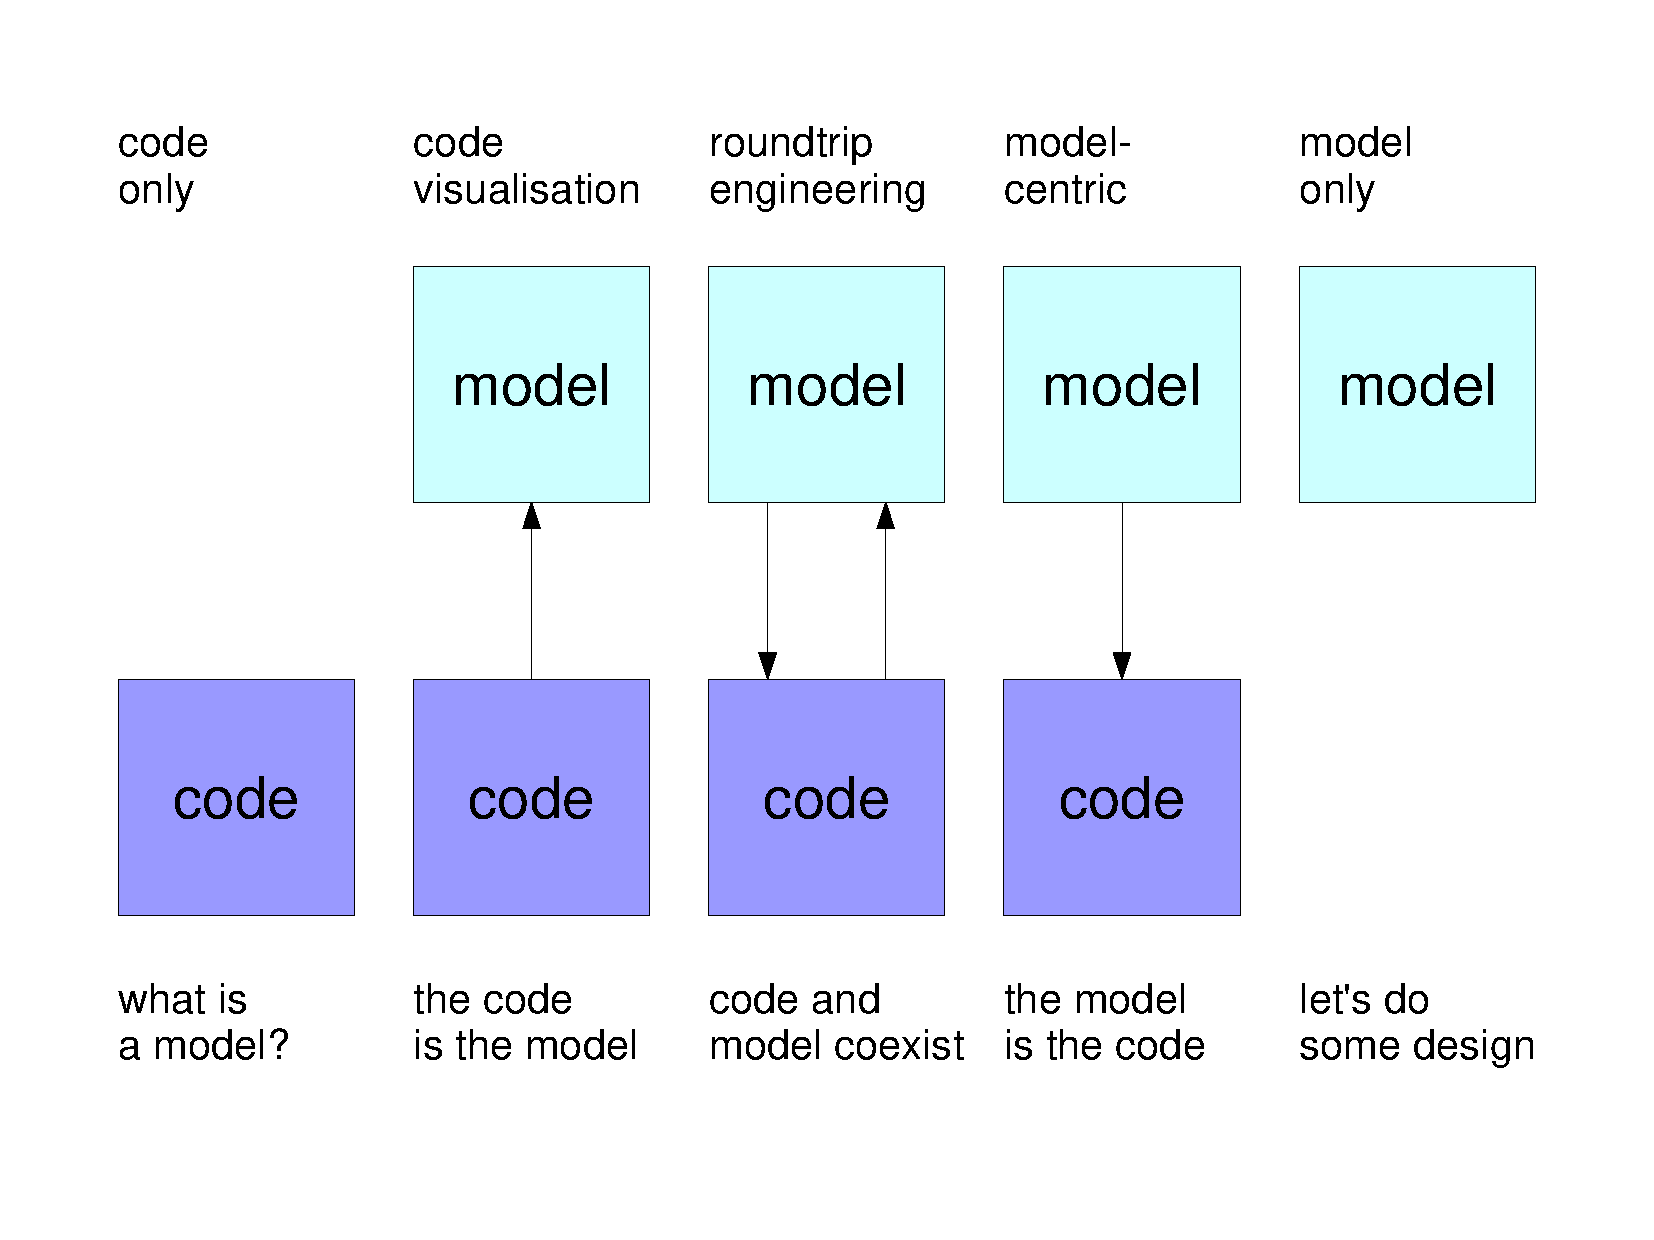
\includegraphics[scale=0.3,angle=-90]{graphic/modelcode.pdf}
        \caption{Model-Code Synchronisation \cite[diagram by John Daniels]{brown2004}}
        \label{modelcode_figure}
    \end{center}
\end{figure}

Alan Brown writes \cite{brown2004}: \textit{One useful way to characterise current
practice is to look at the different ways in which the models are synchronized
with the source code they help describe.} Figure \ref{modelcode_figure} shows
the spectrum of modelling approaches in use today. The different categories
\cite{brown2004} are:

%
% $RCSfile: code_only.tex,v $
%
% Copyright (C) 2002-2008. Christian Heller.
%
% Permission is granted to copy, distribute and/or modify this document
% under the terms of the GNU Free Documentation License, Version 1.1 or
% any later version published by the Free Software Foundation; with no
% Invariant Sections, with no Front-Cover Texts and with no Back-Cover
% Texts. A copy of the license is included in the section entitled
% "GNU Free Documentation License".
%
% http://www.cybop.net
% - Cybernetics Oriented Programming -
%
% http://www.resmedicinae.org
% - Information in Medicine -
%
% Version: $Revision: 1.1 $ $Date: 2008-08-19 20:41:05 $ $Author: christian $
% Authors: Christian Heller <christian.heller@tuxtax.de>
%

\subsubsection{Code Only}
\label{code_only_heading}

\begin{itemize}
    \item[-] almost entire reliance on the code
    \item[-] informal and intuitive modelling of architectural designs
    \item[-] models living on whiteboards, in presentations or the developers' heads
    \item[-] possible use of an \emph{Integrated Development Environment} (IDE)
\end{itemize}

%
% $RCSfile: code_visualisation.tex,v $
%
% Copyright (C) 2002-2008. Christian Heller.
%
% Permission is granted to copy, distribute and/or modify this document
% under the terms of the GNU Free Documentation License, Version 1.1 or
% any later version published by the Free Software Foundation; with no
% Invariant Sections, with no Front-Cover Texts and with no Back-Cover
% Texts. A copy of the license is included in the section entitled
% "GNU Free Documentation License".
%
% http://www.cybop.net
% - Cybernetics Oriented Programming -
%
% http://www.resmedicinae.org
% - Information in Medicine -
%
% Version: $Revision: 1.1 $ $Date: 2008-08-19 20:41:05 $ $Author: christian $
% Authors: Christian Heller <christian.heller@tuxtax.de>
%

\subsubsection{Code Visualisation}
\label{code_visualisation_heading}

\begin{itemize}
    \item[-] alternative modelling using a graphical notation
    \item[-] diagrams aid the understanding of the code's structure or behavior
    \item[-] visual renderings become a direct representation of the code
    \item[-] simultaneous display of code view and model view using
        \emph{Computer Aided Software Engineering} (CASE) tools
\end{itemize}

%
% $RCSfile: roundtrip_engineering.tex,v $
%
% Copyright (C) 2002-2008. Christian Heller.
%
% Permission is granted to copy, distribute and/or modify this document
% under the terms of the GNU Free Documentation License, Version 1.1 or
% any later version published by the Free Software Foundation; with no
% Invariant Sections, with no Front-Cover Texts and with no Back-Cover
% Texts. A copy of the license is included in the section entitled
% "GNU Free Documentation License".
%
% http://www.cybop.net
% - Cybernetics Oriented Programming -
%
% http://www.resmedicinae.org
% - Information in Medicine -
%
% Version: $Revision: 1.1 $ $Date: 2008-08-19 20:41:08 $ $Author: christian $
% Authors: Christian Heller <christian.heller@tuxtax.de>
%

\subsubsection{Roundtrip Engineering}
\label{roundtrip_engineering_heading}

\begin{itemize}
    \item[-] bidirectional exchange between abstract design model and
        implementation code
    \item[-] manual model-to-code transformation, and vice-versa
    \item[-] frequent iterations as errors are detected
    \item[-] considerable discipline necessary to keep models synchronized
    \item[-] automated recognition of generated versus user-defined code by
        \emph{Roundtrip Engineering} (RTE) tools (for example by placing markers
        in the code)
\end{itemize}

%
% $RCSfile: model_centric.tex,v $
%
% Copyright (C) 2002-2008. Christian Heller.
%
% Permission is granted to copy, distribute and/or modify this document
% under the terms of the GNU Free Documentation License, Version 1.1 or
% any later version published by the Free Software Foundation; with no
% Invariant Sections, with no Front-Cover Texts and with no Back-Cover
% Texts. A copy of the license is included in the section entitled
% "GNU Free Documentation License".
%
% http://www.cybop.net
% - Cybernetics Oriented Programming -
%
% http://www.resmedicinae.org
% - Information in Medicine -
%
% Version: $Revision: 1.1 $ $Date: 2008-08-19 20:41:07 $ $Author: christian $
% Authors: Christian Heller <christian.heller@tuxtax.de>
%

\subsubsection{Model Centric}
\label{model_centric_heading}

\begin{itemize}
    \item[-] sufficiently detailed system models enable the generation of full
        system implementations
    \item[-] models include representations of persistent- and non-persistent
        data, business logic, presentation elements and more
    \item[-] interfaces to legacy systems and various services
    \item[-] specialized tools generate particular (constrained) styles of
        applications, in an automated process
\end{itemize}

%
% $RCSfile: model_only.tex,v $
%
% Copyright (C) 2002-2008. Christian Heller.
%
% Permission is granted to copy, distribute and/or modify this document
% under the terms of the GNU Free Documentation License, Version 1.1 or
% any later version published by the Free Software Foundation; with no
% Invariant Sections, with no Front-Cover Texts and with no Back-Cover
% Texts. A copy of the license is included in the section entitled
% "GNU Free Documentation License".
%
% http://www.cybop.net
% - Cybernetics Oriented Programming -
%
% http://www.resmedicinae.org
% - Information in Medicine -
%
% Version: $Revision: 1.1 $ $Date: 2008-08-19 20:41:07 $ $Author: christian $
% Authors: Christian Heller <christian.heller@tuxtax.de>
%

\subsubsection{Model Only}
\label{model_only_heading}

\begin{itemize}
    \item[-] models aid the understanding of a business domain, or the analysing
        of a proposed architecture
    \item[-] models used as basis for discussion, communication and analysis
        among project teams within- or across organisations
    \item[-] establishment of a shared vocabulary and set of concepts among
        disparate teams
    \item[-] model-disconnected (outsourced) implementation of systems
\end{itemize}


Considering the developments of the last decades but especially recent years,
the modelling trend clearly goes \emph{left-to-right}, with respect to figure
\ref{modelcode_figure}, that is from \emph{Code only-} to more \emph{Model-centric}
approaches. The emerge of the \emph{Model Driven Architecture} (MDA) (section
\ref{model_driven_architecture_heading}) is one sign therefore. Yet although
these efforts certainly contribute to easier and faster development, less
inter-dependencies within systems, better documentation and clearity of source
code, improved maintenance and more -- the gap between \emph{Design-} and
\emph{Implementation} phase, within a \emph{Software Engineering Process} (SEP)
(chapter \ref{software_engineering_process_heading}), remains. By introducing a
new knowledge schema (chapter \ref{knowledge_schema_heading}), this work wants
to conclusively close gap number \emph{2} (with respect to figure
\ref{gaps_figure} of section \ref{abstraction_gaps_heading}) and provide a
model-only approach.
